\clearpage
\subsubsection{凸包法}
\label{subsubsec:lab4-task1-convex-hull}

\paragraph{使用SageMath建立完整凸包}

凸包法先从DDT、LAT的非零位置提取合法点，在八维实数空间中构造其凸包，再把凸包的H表示转换成线性约束。实验分为建立凸包和求解两个步骤：\texttt{build\_hull.py}在WSL Arch中使用SageMath计算约束，\texttt{convex\_hull.py}在Windows的\texttt{uv}环境中读取约束并调用Gurobi。

建立凸包时，程序将合法输入输出对编码为八位向量，使用\texttt{QQ}进行精确有理数计算，并分别提取不等式和等式：
\begin{lstlisting}
points = [bits(a, b) for a in range(SIZE) for b in range(SIZE)
          if table[a][b] != 0]
hull = Polyhedron(vertices=points, base_ring=QQ)

hrep = {
    "inequalities": sorted(integer_row(row)
                           for row in hull.inequalities_list()),
    "equations": sorted(integer_row(row)
                        for row in hull.equations_list()),
}
\end{lstlisting}

Sage输出的每行系数按$[c_0,c_1,\ldots,c_8]$排列，第一项为常数，对应$c_0+\sum_{j=0}^{7}c_{j+1}z_j\ge0$，等式使用相同的系数顺序。\footnote{SageMath多面体构造与H表示说明：\url{https://doc.sagemath.org/html/en/reference/discrete_geometry/sage/geometry/polyhedron/constructor.html}。}为便于JSON保存和后续整数计算，\texttt{integer\_row()}先乘以各系数分母的最小公倍数，再约去整数系数的最大公因数。整个过程使用正数缩放，保持不等式方向。

两组完整H表示保存在\texttt{hull\_constraints.json}中，顶层键为\texttt{DDT}和\texttt{LAT}，各自包含\texttt{inequalities}与\texttt{equations}两个系数数组。由于文件位于Windows工作目录，WSL通过\texttt{/mnt/d/}访问并生成文件后，Windows端可以直接读取相同数据。

\paragraph{贪心筛选与Gurobi建模}

完整H表示可以准确描述凸包，但本任务最终只检查二进制点，因此进一步按每条不等式排除非法点的能力进行筛选。程序保留全部等式，将仍满足等式的非法点编号存入\texttt{remaining}，再用\texttt{pool}记录每条候选不等式能够排除的点集。贪心选择的核心循环为：
\par\noindent\begin{minipage}{\linewidth}
\begin{lstlisting}
while remaining:
    row = max(pool, key=lambda item: len(pool[item] & remaining),
              default=None)
    if row is None or not (pool[row] & remaining):
        raise RuntimeError("Incomplete illegal-point coverage")
    chosen.append(row)
    remaining.difference_update(pool.pop(row))
\end{lstlisting}
\end{minipage}\par

其中\texttt{linear\_form(row,point)}计算该行系数在指定点上的值。值小于0表示点违反该不等式，因而可以被排除。候选系数按字典序排列，所以并列时选择顺序固定。每次保留的不等式均来自完整凸包，且筛选结束时所有非法点都已被排除，因此约简后的二进制可行点集仍与原合法点集一致。

最后建立8个二进制变量，将全部等式以$h(z)=0$、筛选后的不等式以$h(z)\ge0$加入Gurobi，再按统一解池设置枚举全部可行点。

\paragraph{实验结果与分析}

SageMath计算完整凸包的输出如图~\ref{fig:lab4-task1-hull-build}所示。
\begin{figure}[H]
    \centering
    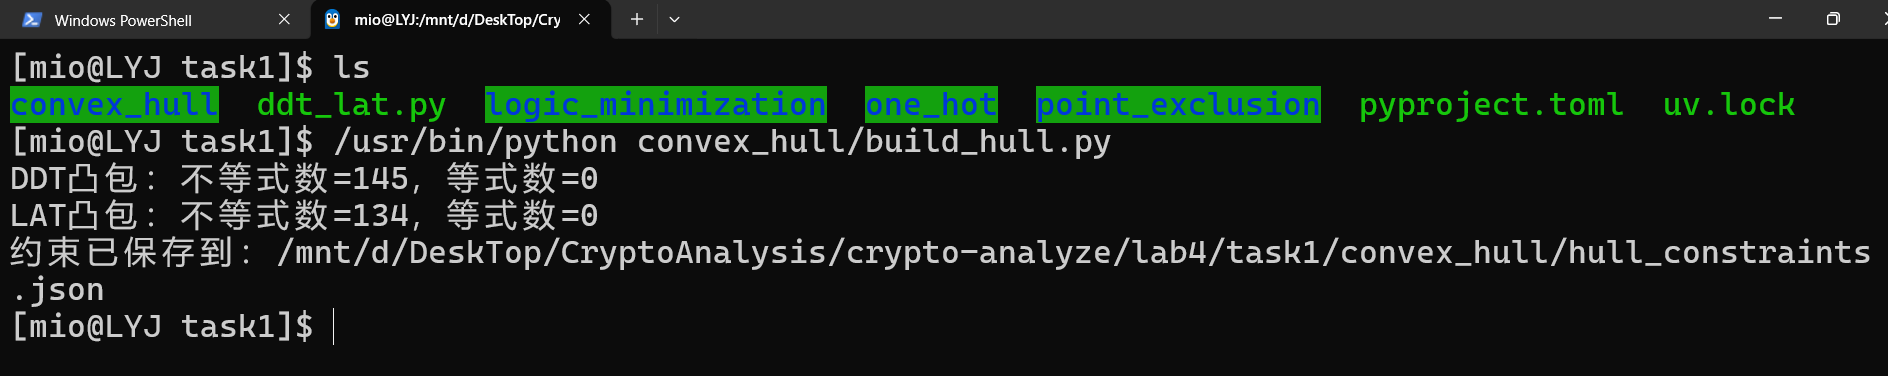
\includegraphics[width=\textwidth]{figures/task1/hell_model.png}
    \caption{SageMath建立DDT、LAT合法点集凸包并保存H表示}
    \label{fig:lab4-task1-hull-build}
\end{figure}

DDT凸包共有145条不等式，LAT凸包共有134条不等式，两者等式数均为0。这与两组合法点集的仿射维数均为8相符。整数化后的约束与直接计算表进行核对时，完整H表示保留的二进制点分别为72个和122个，覆盖全部非零位置。

读取JSON并进行贪心筛选后，Gurobi运行结果如图~\ref{fig:lab4-task1-convex-hull}所示。
\begin{figure}[H]
    \centering
    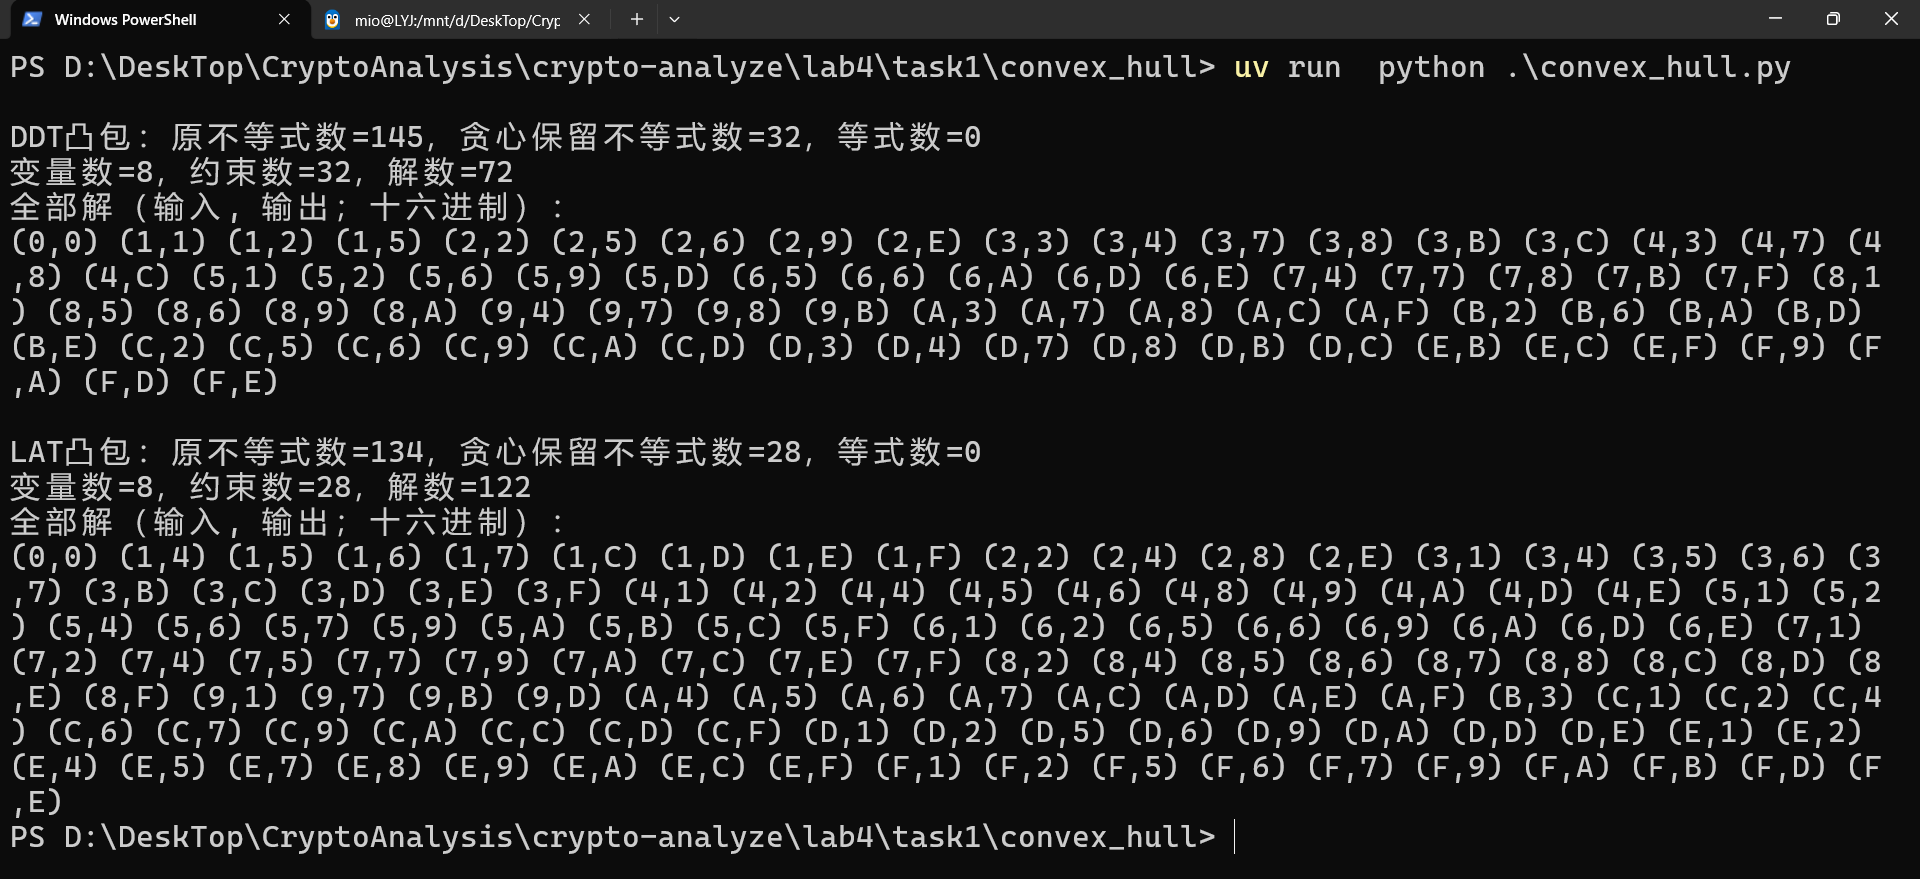
\includegraphics[width=\textwidth]{figures/task1/Grubi_solve3_covex_hell.png}
    \caption{凸包约束经贪心筛选后的Gurobi全解枚举结果}
    \label{fig:lab4-task1-convex-hull}
\end{figure}

DDT模型从145条不等式中保留32条，LAT模型从134条中保留28条。由于没有等式，最终加入Gurobi的约束数分别就是32和28，两种模型的变量数均为8。枚举得到的72个差分输入输出对与122个线性掩码对，与前面三种方法及原始DDT、LAT的非零位置完全一致。

进一步对全部256个二进制点逐一代入约束，完整H表示和筛选后的约束均没有遗漏合法点，也没有保留非法点，说明约束读取、整数化和贪心筛选过程保持了二进制解集。这里的32条和28条约束用于描述合法二进制点；筛选后的连续可行区域可能大于完整凸包，贪心选择也不保证约束数量全局最少。
